\section*{Источники и решения}

\subsubsection*{Укрепление сетки}

Эту интересную (и, возможно, практически полезную) головоломку подкинул мне геометрический гуру Боб Коннелли из Корнеллского университета; она основана на работе Этана Болкера и Генри Крапо \cite{8}.


\begin{figure}[ht!]
\centering
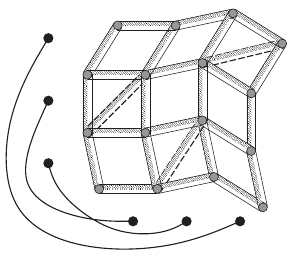
\includegraphics[scale=1]{pics/lattice2}
\caption{Недоукреплённая сетка и её граф.}
\label{pic:lattice2}
\end{figure}

\begin{figure}[t!]
\centering
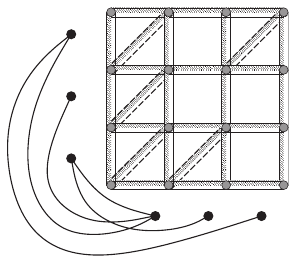
\includegraphics[scale=1]{pics/lattice3}
\caption{Полностью укреплённая сетка и её граф.}
\label{pic:lattice3}
\end{figure}

Задачу полезно перевести на язык графов, но не самым очевидным образом (не нужно смотреть на граф с вершинами в сочленениях стержней).
Предположим, что скобы жёсткости уже расставлены.
Рассмотрим граф $G$, вершины которого соответствуют строкам и столбцам сетки.
Каждое ребро в $G$ соответствует строке и столбцу, пересекающимся по закреплённой клетке, так что число рёбер в $G$ равно числу поставленных скоб.
Сетка с рис. \ref{pic:lattice1}, показана снова на рис. \ref{pic:lattice2}, но уже с её графом.

Предположим, что некоторая строка смежна в $G$ с некоторым столбцом.
Тогда вертикальные стержни этой строки перпендикулярны горизонтальным стержням этого столбца.
Если $G$ --- связный граф (то есть любые две вершины в нём соединимы путём), то все горизонтальные стержни перпендикулярны всем вертикальным.
Таким образом, все горизонтальные стержни параллельны друг другу,
также параллельны и все вертикальные.
Теперь ясно, что сетка жёсткая.

С другой стороны, предположим, что граф несвязен.
Пусть $C$ --- его \emph{компонента}, то бишь связный кусок $G$, рёбра из которого не идут к остальным вершинам $G$.
Тогда ничто не мешает любому вертикальному стержню в строке $C$ или любому горизонтальному стержню в столбце $C$ поворачиваться относительно остальных стержней в сетке.

Таким образом, жёсткость сетки в точности означает связность графа $G$.
Поскольку $G$ имеет $2n$ вершин, то для его связности нужно как минимум $2n - 1$ ребро.
(Если это для вас новость, воспользуйтесь индукцией по числу вершин.)
Следовательно, чтобы сделать сетку жёсткой, нужны как минимум $2n - 1$ скоб.

Обратите внимание, что скобы нельзя ставить где попало.
На рисунке 21 показана полностью закреплённая сетка $3 \times 3$, и её граф.
Попробуйте подсчитать, сколькими способами можно укрепить сетку $3 \times 3$, используя минимальное число скоб  (пять штук).
Есть теорема в теории графов о том, что у каждого связного графа есть \emph{остовное дерево}, т.е. связный подграф с минимальным числом рёбер.
Она позволяет сделать следующий вывод: \emph{если закреплены больше чем $2n - 1$ клеток и сетка жёсткая, то можно удалить все скобы, кроме $2n - 1$, сохранив жёсткость.}%
\footnote{Про число таких способов можно прочитать в квантовской заметке переводчика \cite{petrunin-2018}. \pr}

\subsubsection*{Путешествие по острову}

Эта головоломка из уже упомянутой выше книги «Московские математические олимпиады» Г. А. Гальперина и А. К. Толпыго \cite{23}; её вариант удостоился чести попасть на веб-страницу «The Puzzle Toad» \cite{bohman-pikhurko-frieze-sleator}.
%???не смог лучше сказать...

Между перекрёстками текущее состояние Алоисия характеризуется тройкой, состоящей из ребра, на котором он находится, направления движения и типа последнего поворота (вправо или влево).
Эта тройка полностью определяет как будущие, так и прошлые положения Алоисия.
Поскольку таких троек конечное число, настанет момент, когда Алоисий впервые попадёт в одну и ту же тройку, и это может произойти только на его стартовом ребре!


\subsubsection*{Провода под Гудзоном}

Вариант этой головоломки рекламировал Мартин Гарднер,
иногда её называют задачей Грэма --- Нолтона.
Для электриков это просто задача идентификации кабельных линий.
В версии Гарднера можно было замыкать любое число проводов на любом берегу и также проверять их на любом берегу.
Следующее решение было предложено Роландом Шпрагом в его книге \cite{54}, а также в недавней статье трёх молодых специалистов по информатике Навина Гойала, Сачина Лодхи и Муту Мутукришнана \cite{33}.
Оно удовлетворяет нашим дополнительным ограничениям и требует только двух операций на каждом конце (таким образом, потребуются три переправы через реку, не считая дополнительной операции размыкания проводов перед использованием).
Однако решение не единственно, и если ваше трёхпереправное решение отличается, то оно может быть ничуть не хуже.

Пусть концы проводов на западном берегу помечены как $w_1$, $w_2, \z\dots, w_{50}$,
а на на восточном как $e_1, \dots, e_{50}$ .
При первом посещении западного берега соединим $w_1$ с $w_2$, $w_3$ с $w_4$, $w_5$ с $w_6$ и так далее, но последнюю пару $w_{49}$ и $w_{50}$ соединять не будем.
Затем проверим провода на восточном берегу, пока не найдём все пары.
Например, мы могли бы обнаружить, что $e_4$ соединён с $e_{29}$, $e_2$ с $e_{15}$, $e_8$ с $e_{31}$ и так далее, а концы $e_{12}$ и $e_{40}$ остались без пар.
Затем мы едем на западный берег, рассоединив все пары, соединяем $w_2$ с $w_3$, $w_4$ с $w_5$ и так далее, оставив $w_1$ и $w_{50}$ без соединения.
Возвращаемся на восточный берег и опять находим все пары.
Продолжая пример, пусть $e_{12}$ теперь соединён с $e_{15}$, $e_{29}$ с $e_2$, и $e_4$ с $e_{31}$, а концы $e_{40}$ и $e_8$ остались без пар.

Удивительно, но этих действий достаточно!

Тот восточный конец провода, который имел пару в первый раз, но не во второй (в нашем примере это $e_8$), должен соответствовать $w_1$.
Следовательно, восточный конец провода, с которым $e_8$ был спарен в первый раз (у нас это $e_{31}$), должен соответствовать $w_2$.
Но тогда $w_3$ должен соответствовать восточному концу провода, с которым $e_{31}$ был спарен во второй раз, а именно $e_4$.
Продолжая таким образом, мы находим, что $w_4$ соответствует $e_{29}$ (п\'{а}рному к $e_4$ на первом круге), $w_5$ соответствует $e_2$ (п\'{а}рному к $e_{29}$ на втором круге) и так далее. В конце мы видим, что $w_{50}$ соответствует $e_{40}$.

Аналогично можно решить задачу для любого чётного числа проводов. Если же число проводов (скажем, $n$) нечётно, то в первый раз можно оставить без пары только $w_n$, а во второй --- только $w_1$, и всё сработает примерно так же.

\subsubsection*{Жуки на четырёх прямых}

Эта головоломка мне досталась от Мэтта Бэйкера из Технологического института Джорджии.
Иногда её называют \emph{задачей четырёх путешественников};
её можно увидеть на сайте «Cut the knot» \cite{cut-the-knot}.

В наиболее изысканном решении, которое мне известно, требуется выйти из плоскости в пространство, добавив ось времени.
Предположим, что встречаются все, кроме (возможно) третьего и четвёртого жука.
Проведём ось времени перпендикулярно плоскости с жуками, и пусть $g_i$ --- график $i$-го жука в пространстве.
Поскольку каждый жук ползёт с постоянной скоростью, каждый такой график --- прямая линия; его проекция на плоскость с жуками --- та прямая, по которой ползёт жук.
Два жука встречаются тогда (и только тогда), когда их графики пересекаются.

Прямые $g_1$, $g_2$ и $g_3$ находятся в одной плоскости, так как они попарно пересекаются. То же самое относится и к тройке  $g_1$, $g_2$ и $g_4$.
Следовательно, все 4 графика лежат в одной плоскости.
Конечно же, $g_3$ и $g_4$ не параллельны, ведь не параллельны их проекции.
Таким образом, эти две прямые обязаны пересечься в своей плоскости,
а это и значит, что третий жук встретит четвёртого.

\begin{addedbytheeditors}
Эта задача предлагалась на Московской математической олимпиаде 1958 года \cite[Задача 78148]{problems.ru}.
\pr
\end{addedbytheeditors}

\subsubsection*{Пауки на кубе}

У этой головоломки тот же источник, что и у «Путешествия по острову» выше.

\begin{figure}[ht!]
\centering
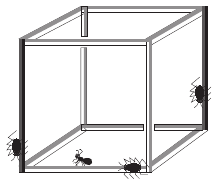
\includegraphics[scale=1]{pics/cube}
\caption{Два чёрных ребра под контролем, и муравей ловится в серой зоне.}
\label{pic:cube}
\end{figure}

Для поимки муравья можно заставить двух пауков охранять по одному ребру.
Для охраны ребра $PQ$ паук сначала выгоняет с него муравья, если это необходимо, а затем бегает по ребру так, что он всегда хотя бы в три раза ближе к $P$ (и к $Q$), чем муравей.
Это возможно, ведь если запрещено использовать ребро $PQ$, то любой путь от $P$ до $Q$ вдоль рёбер куба по крайней мере втрое длиннее самого ребра.

Если охранять два \emph{противоположных} ребра (другие варианты также работают), то оставшаяся часть куба (без этих рёбер и их концов) не имеет циклов (см. рис. \ref{pic:cube}).
Значит, третий паук сможет преследовать муравья до конца охраняемого ребра, где тот и встретит свою грустную участь.

\subsubsection*{Вменяемые мыслители}

Эту головоломку мне предложил Саша Разборов из Института перспективных исследований;
с его слов я знаю, что она была кандидатом на Международную математическую олимпиаду, однако была отвергнута как слишком сложная.
Она была рассмотрена и решена в статье Э. Голеса и Х. Оливоса \cite{31}.

Нам надо доказать, что мнения стабилизируются или будут меняться с периодом в две недели.
Между каждой парой друзей нарисуем пару стрелок, по одной стрелке в каждом направлении.
Назовём стрелку \emph{обидной}, если мнение перевёртовца в начале стрелки отличается от мнения его друга на конце стрелки на \emph{следующей неделе}.

Рассмотрим стрелки, выходящие от перевёртовца Клайда на неделе $t - 1$, во время которой Клайд выступает (скажем) за торговый центр.
Предположим, что из них $m$ обидных.
Если Клайд всё ещё (или снова) за торговый центр на неделе $t + 1$, то число  $n$ обидных стрелок, указывающих на Клайда на неделе $t$, будет в точности равно~$m$.

Однако, если Клайд против торгового центра на неделе $t + 1$, то $n$ будет строго меньше $m$, так как большинство его друзей были против торгового центра на неделе $t$.
Следовательно, большинство стрелок от Клайда были обидными на неделе $t - 1$, а на неделе $t$ только меньшинство обидных стрелок направлены к Клайду.

Всё сказанное останется верным и если Клайд был против торгового центра на неделе $t - 1$.

Но \emph{каждая} стрелка начинается у \emph{кого-то} на неделе $t - 1$ и заканчивается у кого-то на неделе $t$.
Таким образом, общее число обидных стрелок между неделями $t - 1$ и $t$ не увеличивается и даже строго уменьшается, за исключением случая, когда каждый перевёртовец имел такое же мнение на неделе $t - 1$, как и на неделе $t + 1$.

Общее число обидных стрелок (в данную неделю) не может бесконечно уменьшаться.
В итоге оно достигнет значения, с которого уже не опустится.
В этот момент каждый перевёртовец либо сохранит своё мнение навсегда, либо будет менять его туда-сюда каждую неделю.

\medskip

Задачу можно значительно обобщить, например, добавив веса вершинам (это означает, что мнения одних ценнее других), или разрешив петли (то есть разрешив учитывать своё текущее мнение), введя механизмы разрешения конфликтов и даже установив различные пороги для смены мнений «за» и «против».

\subsubsection*{Лемминг на шахматной доске}

Эту замечательную головоломку придумал Кевин Пурбху, ещё будучи старшеклассником в Торонто.
С тех пор он защитил диссертацию по математике в Университете Калифорнии в Беркли и вернулся в Торонто в качестве доцента кафедры комбинаторики Университета Ватерлоо.
Сам я узнал головоломку от Рави Вакила из Стэнфордского университета.

Лемминг действительно обречён.
Один из способов это понять (найденный независимо Вакилом и мной) --- представить, что лемминг может перемещаться на любую соседнюю клетку, но должен при этом повернуться в направлении стрелки, которую он там обнаружит.
Лемминг не может повернуться на 360°, обойдя клетки по циклу;
ведь если бы он мог, то можно уменьшать такой цикл, пока не придём к противоречию.
Но настоящий лемминг, если он хочет остаться на доске, в конечном итоге должен обойти цикл, и когда это произойдёт, ему придётся повернуть на 360°.

Собственное решение Пурбху, с его школьных лет, использует индукцию.
Если лемминг остаётся на доске, он, как мы уже отметили, должен будет обойти цикл.
Пусть $C$ --- цикл наименьшей возможной площади (на любой доске), на котором это может произойти; будем считать, что лемминг обходит его по часовой стрелке.
Обрежем всю доску до $C$ и того, что он окружает.
Затем повернём все стрелки на 45° по часовой стрелке.
Это приведёт нас к меньшему циклу!

\begin{addedbytheeditors}
Нехитрая техника позволяет свести головоломку к следующему утверждению про векторные поля: \emph{Векторное поле без нулей на плоскости не имеет замкнутых интегральных линий.}
Решение получается сложней, но, возможно, полезней.\pr
\end{addedbytheeditors}
